\section{Learning entry size with contextual bandits}\label{sec:11}

We use direct policy search to learn a contextual sizing policy that maximizes historical portfolio Sharpe. The rule fixes direction and contracts; the bandit chooses 50\%, 75\% or 100\% exposure. CEM optimizes the put policy.


\subsection*{Put pairs: group observations, then search size assignments}

Each monthly regression tree uses completed examples from the preceding 18 months. Its target is cumulative full-size profit above cash; splits reduce prediction error across 27 inputs. At most eight leaves define states. With n examples, minimum leaf count is max(8, min(63, floor(n/8))); fewer than 16 use full size.


\begin{figure}[!htbp]\centering
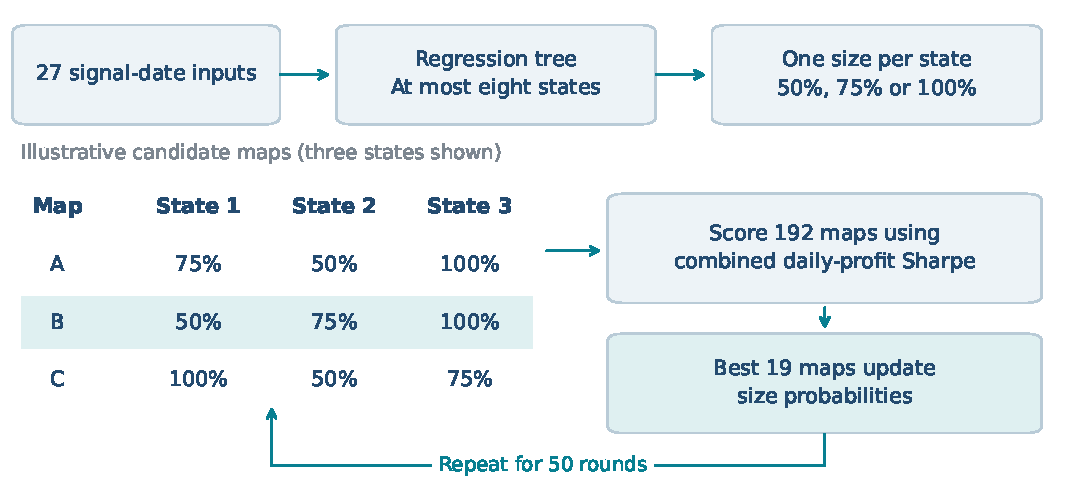
\includegraphics[width=\linewidth]{entry_policy.pdf}
\caption{The original tree/CEM construction. The three-state maps illustrate candidates; actual trees have up to eight states. Each candidate selects action-specific completed paths; the best 19 update sampling probabilities. The retained map sizes next month's proposals.}\label{fig:entry-policy}
\end{figure}

For completed example i, p denotes its profit above cash on day d at size a. Each size has its own rounded contracts and simulated hedge path. A map assigns one size to each tree state. We sum its daily paths, retaining overlapping positions and zero-profit sessions, and score the result:


\begin{equation*}g_d(m)=\sum_i p_{i,d}(a_{\ell(x_i)}),\qquad\widehat S_{\rm train}(m)=\sqrt{252}\,\overline{g}/s_g.\end{equation*}

CEM \cite{deboer2005} updates size probabilities toward the best 19 of 192 candidate maps for 50 rounds. Constant maps and the incumbent are anchors. This standalone-path training score differs from funded-account Sharpe: replay additionally applies shared cash, inventory and admission.


\subsection*{Straddles: the same decision with ridge-score contexts}

The straddle bandit fits a 60-month ridge model to completed full-size profit, using 14 inputs and requiring 128 examples. The inputs include IV, RV-IV memory, VIX and a separate fixed-half paper portfolio's recent performance. Score terciles define three states. We enumerate all 27 size maps and retain the highest training Sharpe. Insufficient history uses half size. Both learners use completed outcomes; Appendix~\ref{app:b} provides exact fitting details.
